\subsection{Decision presentation pattern} \label{odp_decision_presentation}
The outcome of a decision might deviate from the expectations of the decision-maker when the information maturity-level is low. This deviation is not a big problem when the impact of the decision on the organisation is low. However, when the impact of the decision on the organisation is high, the decision-maker wants more certainty that the decision reaches the expected outcome. There is a consensus on the benefits of evidence-based decision-making. However, \cite{DM03} and \cite{DM07} also raise the need for more research to prove its effectiveness.

\begin{center}
\large\color{document}{The decision presentation pattern helps decision-makers to make evidence-based decisions by presenting the information maturity-level.} 
\end{center}

The decision presentation pattern achieves this goal by enabling the decision-maker to understand the maturity-level of the decision-relevant information. We give decision-makers two options when we present the information maturity-level:
\begin{enumerate}
\item Accept the status of the decision-relevant information.
\item Elaborate further on the decision-relevant information.
\end{enumerate}

We enable the decision-maker to understand which information requires more elaboration. This elaboration can increase the completeness and reliability of the information. We present three dashboards for the decision-maker. The first dashboard presents the information maturity-level and evidence spread for all the decision-relevant information. The second dashboard presents the information maturity-level for the completeness, reproducibility, consensus, and conflict patterns. The third dashboard presents the maturity-levels per individual. 

Figure \ref{fig:04_Presentation_Components} presents a navigation concept for the three dashboards. The decision-maker can browse from the first dashboard to the second dashboard, from the second dashboard to the third dashboard, and from the first dashboard to the third dashboard. The context of the third dashboard changes depending on the origin of the decision-maker. For example, if the decision-maker browses from dashboard two to dashboard three using the completeness maturity-level, dashboard three presents the completeness of the decision-relevant information per individual.

\begin{figure}[H]
\centering
  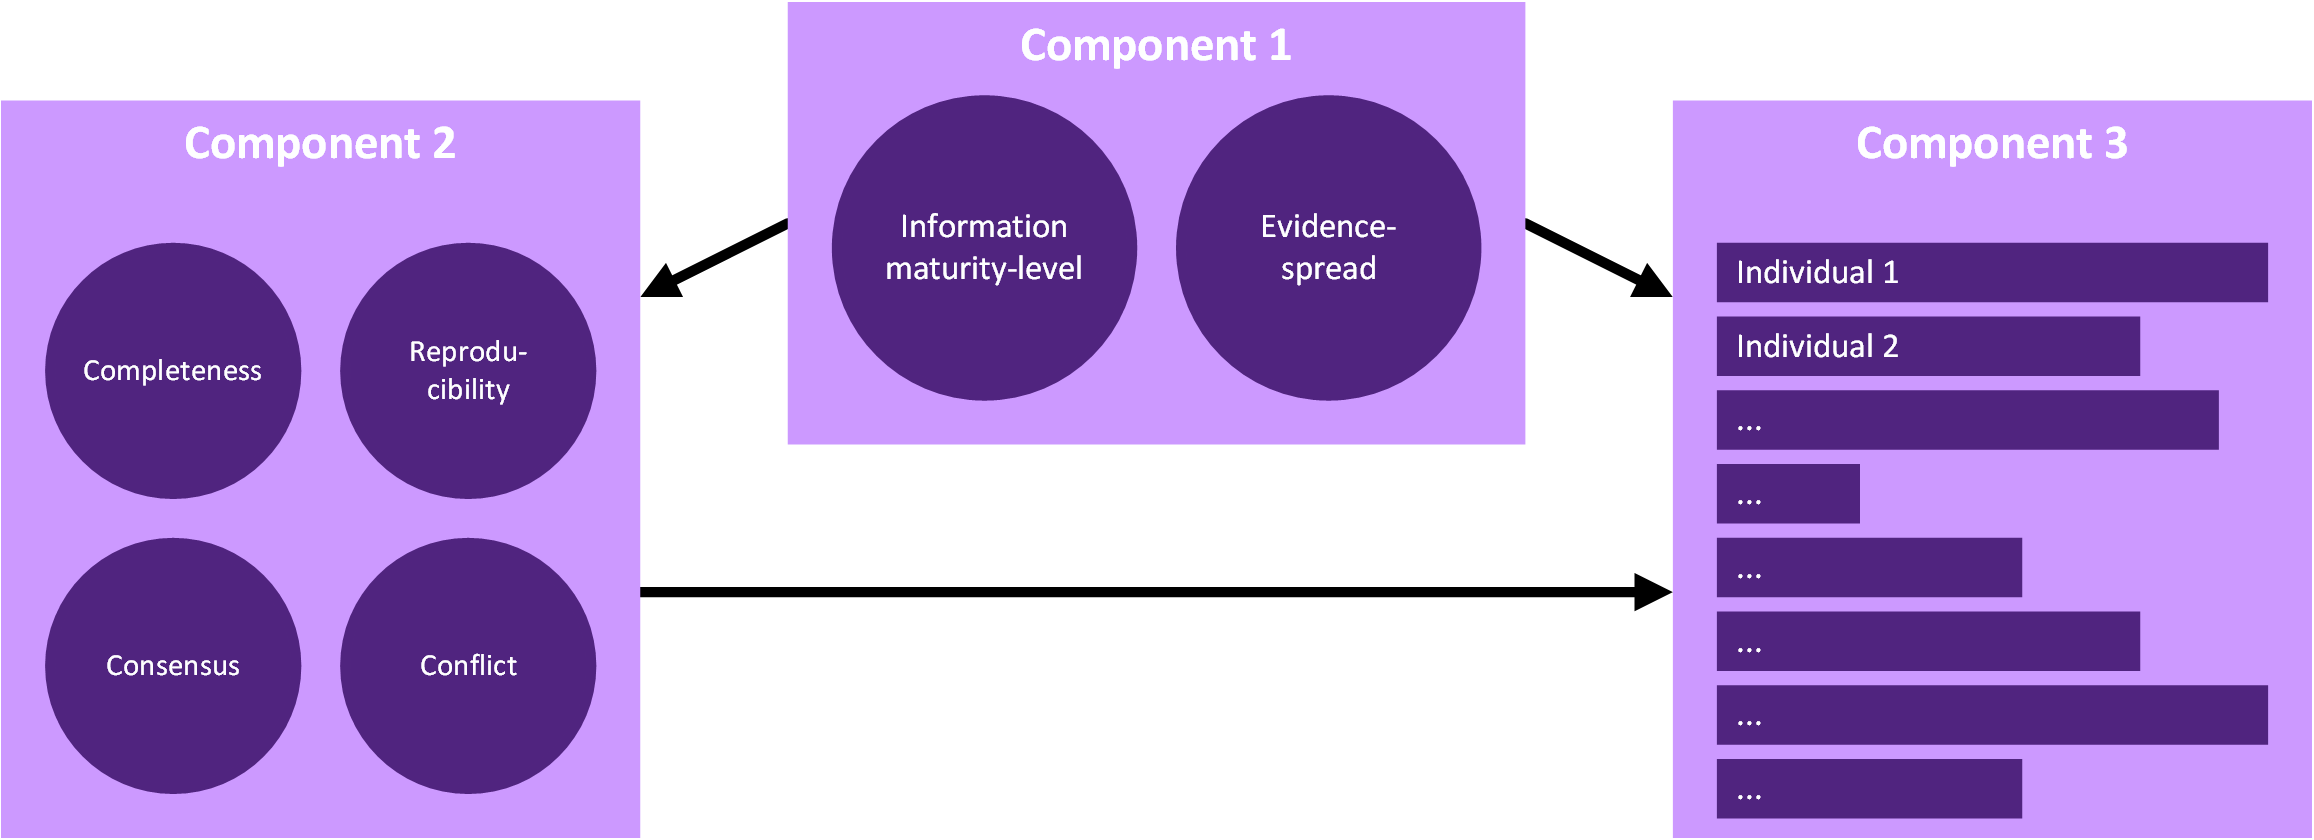
\includegraphics[width=16cm]{../../Images/04_Contribution/04_Presentation_Components.png}
  \caption{The three presentation dashboards that allow a decision-maker to understand the information-maturity level and evidence-spread.}
  \label{fig:04_Presentation_Components}
\end{figure} 

\subsubsection{Dashboard 1: Consolidated information maturity-level and evidence spread} \label{odp_maturity_evidence_spread}
The goal of the first dashboard is to help decision-makers to decide if the information maturity-level and evidence-spread are acceptable in the context of the specific decision. We determine an average information maturity-level and evidence-spread across the decision-relevant root individuals. Figure \ref{fig:root_information_target_1} repeats the definition of the root, information, and target individuals.

\begin{figure}[H]
\centering
  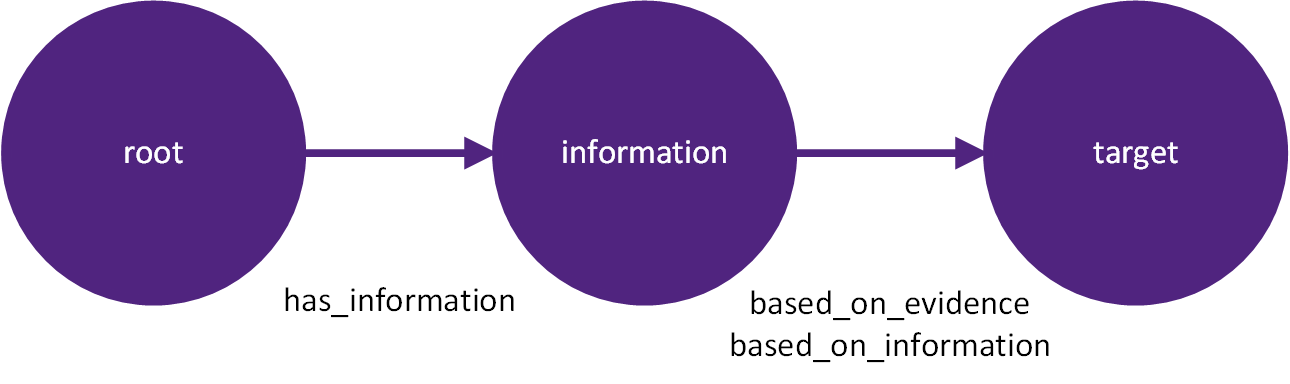
\includegraphics[width=10cm]{../../Images/04_Contribution/04_root_information_target.png}
  \caption{The $root$, $in{\f}ormation$, and $target$ individuals in n-ary relation.}
  \label{fig:root_information_target_1}
\end{figure}

We need to know the maximum number of violations before we can determine the information maturity-level. The maximum number of violations depends on the decision-relevant root individuals. We create a set $RI$ that contains the decision-relevant root individuals. The contents of the set $RI$ depend on the context of the decision. Therefore, we cannot define $RI$ as part of the pattern.  

\paragraph{Maximum number of violations: Completeness}
The maximum number of violations for the completeness pattern for a specific decision-relevant root individual depends on three things: 
\begin{enumerate}
\item The required $has\_in{\f}ormation\_*$ object properties.
\item The availability of the $data\_value$ and $data\_description$ data properties.
\item The availability of context-specific data properties.  
\end{enumerate}

First, we need to retrieve the $has\_in{\f}ormation\_*$ object properties for a specific decision-relevant root individual independent from the ontology content. We need to extract this information manually from the ontology structure by analysing the $has\_in{\f}ormation\_*$ object properties. We represent this manual extraction process in the function $hi(ri) \Rightarrow \mathbb{N}$. $ri$ represents a decision-relevant root individual.

Second, each $has\_in{\f}ormation\_*$ object property leads us to an individual classified as $Information$. Information individuals require a $data\_value$ and $data\_description$. Therefore, we multiply the output of $hi$ by $2$ and add it to the result. 

Third, adding additional object or data properties to the maximum number of violations for the completeness pattern might be necessary. We use variable $c$ for adding the context-specific violations for each decision-relevant root individual.

Equation \ref{eq:mvi1} returns the maximum number of violations for the completeness pattern considering the decision-relevant root individual $ri$ as a parameter: $mvi_1(ri) \rightarrow \mathbb{N}$.

\begin{equation} \label{eq:mvi1}
mvi_1(ri) = hi(ri) + 2hi(ri) + c
\end{equation}

Equation \ref{eq:mv_1} presents the maximum number of violations for the completeness pattern $mv_1$, considering the set of decision-relevant root individuals $RI$. The decision-relevant root individuals are context-dependent. We define a SPARQL query to extract the decision-relevant root individual per scenario.  

\begin{equation} \label{eq:mv_1}
mv_1(RI) = \sum_{ri \in RI} mvi_1(ri)
\end{equation}

\paragraph{Maximum number of violations: Reproducibility}
The maximum number of violations for the reproducibility pattern depends on the number of information classes that require reproduction. We use the same concept to retrieve the maximum number of violations for the reproducibility as we did for the completeness pattern. 

Equation \ref{eq:mvi2} returns the maximum number of violations for the reproducibility pattern considering the decision-relevant root individual $ri$ as a parameter: $mvi_2(ri) \rightarrow \mathbb{N}$.

\begin{equation} \label{eq:mvi2}
mvi_2(ri) = hi(ri)
\end{equation}

Equation \ref{eq:mv_2} presents the maximum number of violations $mv_2$ for the reproducibility pattern considering the set of decision-relevant root individuals $RI$. 

\begin{equation} \label{eq:mv_2}
mv_2(RI) = \sum_{ri \in RI} mvi_2(ri)
\end{equation}

\paragraph{Maximum number of violations: Consensus}
The maximum number of violations for the consensus pattern depends on the maximum number of used evidence sources in the context of a decision. Each evidence source can generate  one violation. Code sample \ref{SPARQL_CONS_IML_ri} presents a SPARQL query that counts the $Used\_Evidence$ individuals based on the object property $evidence\_used\_for$. $evidence\_used\_for$ is the inverse of $based\_on\_evidence$. 

\begin{lstlisting}[float,language=SPARQL1,caption={The SPARQL query that retrieves the number of individuals that the reasoner classified as $Used\_Evidence$ in the context of a specific root class.},label={SPARQL_CONS_IML_ri}][H]
SELECT (COUNT(DISTINCT ?t) as ?count) 
WHERE 
{
	?r has_information ?i .
	?i based_on_evidence ?t .
	?t rdf:type Used_Evidence .
	FILTER (?r = <ri_1>)
}
\end{lstlisting}

Equation \ref{eq:mvi2} returns the maximum number of violations for the reproducibility pattern considering the decision-relevant root individual $ri$ as a parameter: $mvi_3(ri) \rightarrow \mathbb{N}$. Function $uei(ri) \rightarrow \mathbb{N}$ represents the output of the SPARQL query code sample \ref{SPARQL_CONS_IML_ri} presents.

\begin{equation} \label{eq:mvi3}
mvi_3(ri) = uei(ri)
\end{equation}

We cannot sum the results of the individual violations as there might be duplicates in the results. For example, two information individuals might use the same evidence. When counting the maximum number of violations per individual, the sum would count this evidence as two violations. However, considering one decision, one evidence source can generate up to one violation. Code sample \ref{SPARQL_CONS_IML_RI} presents a new filter that we apply on code sample \ref{SPARQL_CONS_IML_ri}. We add the entire content of the set $RI$ to the filter. This way, we ensure that we get a list of evidence sources that is distinct for the specific decision.

\begin{lstlisting}[float,language=SPARQL1,caption={A new filter that we apply on code sample \ref{SPARQL_CONS_IML_ri}. We add the entire content of the set $RI$ to the filter.},label={SPARQL_CONS_IML_RI}][H]
FILTER (?r = <ri_1> || ?r = <ri_2> || ?r = <ri_x>)
\end{lstlisting}

Equation \ref{eq:mv_3} presents the maximum number of violations $mv_3$ for the reproducibility pattern considering the set of decision-relevant root individuals $RI$. Function $ue(RI) \rightarrow \mathbb{N}$ represents the SPARQL query code sample \ref{SPARQL_CONS_IML_RI} presents.

\begin{equation} \label{eq:mv_3}
mv_3(RI) = ue(RI)
\end{equation}

\paragraph{Maximum number of violations: Conflict}
The conflict pattern detects information individuals that have conflicting evidence using the $conflict\_with\_evidence$ object property. The pattern does not care about the number of conflicting evidence related to an individual. Alternatively, we could have used a similar mechanism as we used for the consensus pattern and detect conflict based on the $disagrees\_with$ object property. However, we solve the violation in the consensus pattern by adding an $agrees\_with$ object property to the evidence. The decision-maker can solve the conflict detected by the pattern by removing conflicting evidence or changing the information. In other words, the consensus pattern uses the $Evidence$ class as the core of the solution, while the conflict pattern uses the $Information$ class as the core of the solution.

The maximum number of conflict violations for a decision-relevant root individual depends on the maximum number of information classes that can be evidence-based. We re-use equation $mvi_2$ to determine the maximum number of conflict violations. Equation \ref{eq:mvi24} presents the maximum number of violations $mvi_4$ for the conflict pattern. 

\begin{equation} \label{eq:mvi24}
mvi_2(ri) = mvi_4(ri) = hi(ri)
\end{equation}

Equation \ref{eq:mv_4} presents the maximum number of violations $mv_4$ for the reproducibility pattern considering the set of decision-relevant root individuals $RI$. $mv_4$ is equal to $mv_2$.

\begin{equation} \label{eq:mv_4}
mv_4(RI) = \sum_{ri \in RI} mvi_4(ri)
\end{equation}

\paragraph{Consolidated information maturity-level}
We calculate the information maturity-level using the number of violations detected on the decision-relevant information and the maximum violations. For example, if an individual requires ten object properties and two data properties to be complete, and it triggers two violations, we define the information maturity-level as $(12-2)/12 = 83\%$. Equation \ref{eq:information_maturity_level} includes function $mv(RI) \Rightarrow \mathbb{N}$. This function calculates the maximum number of violations for the set of decision-relevant information. $av(RI) \Rightarrow \mathbb{N}$ calculates the actual number of violations for the set of decision-relevant information and $iml(RI) \Rightarrow \mathbb{N}$ represents the information maturity-level for the set.

\begin{equation} \label{eq:information_maturity_level}
iml(RI) = \dfrac{mv(RI)-av(RI)}{mv(RI)}
\end{equation}

We can easily retrieve the actual number of violations from, for example, Prot\'eg\'e and the SHACL4P plugin. Figure \ref{fig:04_Presentation_IML_SHACL4P} presents an example for which the defined constraints detected two violations for $Opportunity\_SC2\_Vision\_Contribution$. 

\begin{figure}[H]
\centering
  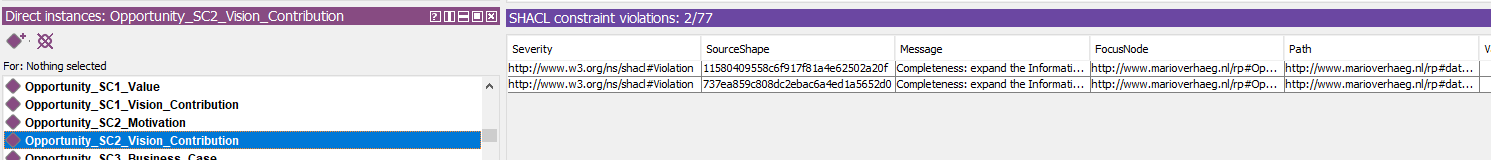
\includegraphics[width=17cm]{../../Images/04_Contribution/04_Presentation_IML_SHACL4P.png}
  \caption{The constraints detect two violations for $Opportunity\_SC2\_Vision\_Contribution$ in Prot\'eg\'e.}
  \label{fig:04_Presentation_IML_SHACL4P}
\end{figure}

Additionally, we need to define the maximum number of violations per decision-relevant root individual and pattern. The maximum number of violations per pattern for a specific individual defines the total maximum number of violations: $mv(RI) = mv_1(RI) + mv_2(RI) + mv_3(RI) + mv_4(RI)$, in which:
\begin{enumerate}
\item $mv_1(RI)$ is the maximum number of violations for the completeness pattern.
\item $mv_2(RI)$ is the maximum number of violations for the reproducibility pattern.
\item $mv_3(RI)$ is the maximum number of violations for the consensus pattern.
\item $mv_4(RI)$ is the maximum number of violations for the conflict pattern
\end{enumerate}

$RI$ represents the set of decision-relevant root individuals.

\paragraph{Evidence spread}
We increase the transparency of the information maturity-level by presenting the evidence spread. For example, a decision entirely based on the evidence type $Stakeholder\_Experience$ might require more elaboration. We use a query to extract the evidence spread from the decision ontology pattern. Within this query, we search for root individuals $ri$ that represent decision-relevant information. The filter in the query accepts multiple root individuals using $||$ the (OR) filter criteria. Code sample \ref{SPARQL_ES} presents the SPARQL query. 

\begin{lstlisting}[float,language=SPARQL1,caption={The SPARQL query that retrieves the evidence spread for decision-relevant information. The SPARQL query counts the individuals that are based on a specific evidence class using type $?t$ of evidence class $?e$.},label={SPARQL_ES}][H]
SELECT ?t (COUNT(DISTINCT ?t) as ?count) 
WHERE 
{
	{
			?ri has_information ?i .
    		?i based_on_evidence ?e .
    		?e rdf:type ?t .
	}
	FILTER(?ri = <ri1> || ?ri = <ri2> || ?rix = <rix> ).
	FILTER(?t != owl:Thing && ?t != Evidence && ?t != Used_Evidence && ?t != Stakeholder_Evidence)
}
GROUP BY ?t
\end{lstlisting}

\paragraph{Overview dashboard}
The goal of the first high-level dashboard is to help the decision-maker answering the question:

\begin{center}
\large\color{document}{Is the information ready for an evidence-based decision?}
\end{center}

This dashboard consists of two charts: the overall information maturity-level and the evidence spread. The information maturity-level helps the decision-maker to understand the quality-level of the information related to this decision. The evidence-spread helps the decision-maker to understand the source of the evidence. The decision-maker needs to find a balance between the information maturity-level and the decision impact, and the evidence-spread and the decision impact. When the impact of a decision is relatively low, the decision-maker might accept a lower information maturity-level and a consolidated evidence-spread. However, when the impact of a decision is relatively high, we expect that decision-makers will require a higher information maturity-level and would like to see a dispersed evidence-spread.

We use a pie-chart to help the decision-maker to understand the mix of evidence-types. The pie-chart is suitable to present relative proportions and percentages \parencite{OTH09}.

We express the information maturity-level as a percentage. Therefore, we use a pie-chart for presenting the information maturity-level as well. Figure \ref{fig:Dashboard_Component_1} presents an example of a dashboard that contains the pie chart presenting the evidence-spread and the information maturity-level. We shorten the time it takes for a decision-maker to consume the information on the dashboard by limiting the number of charts, using data labels to show the actual values, and using a clear legend \parencite{BI09}. Additionally, we use an analogous colour scheme for the evidence spread to ensure the chart appears as one, but the colours are still easily recognisable \parencite{BI10}. The pie chart presenting the information maturity-level uses a different colour scheme, representing \emph{good} (the mature information) and \emph{bad} (the premature information) as \textcolor{LightGreen}{green} and \textcolor{Red}{red}.

\begin{figure}[H]
\centering
  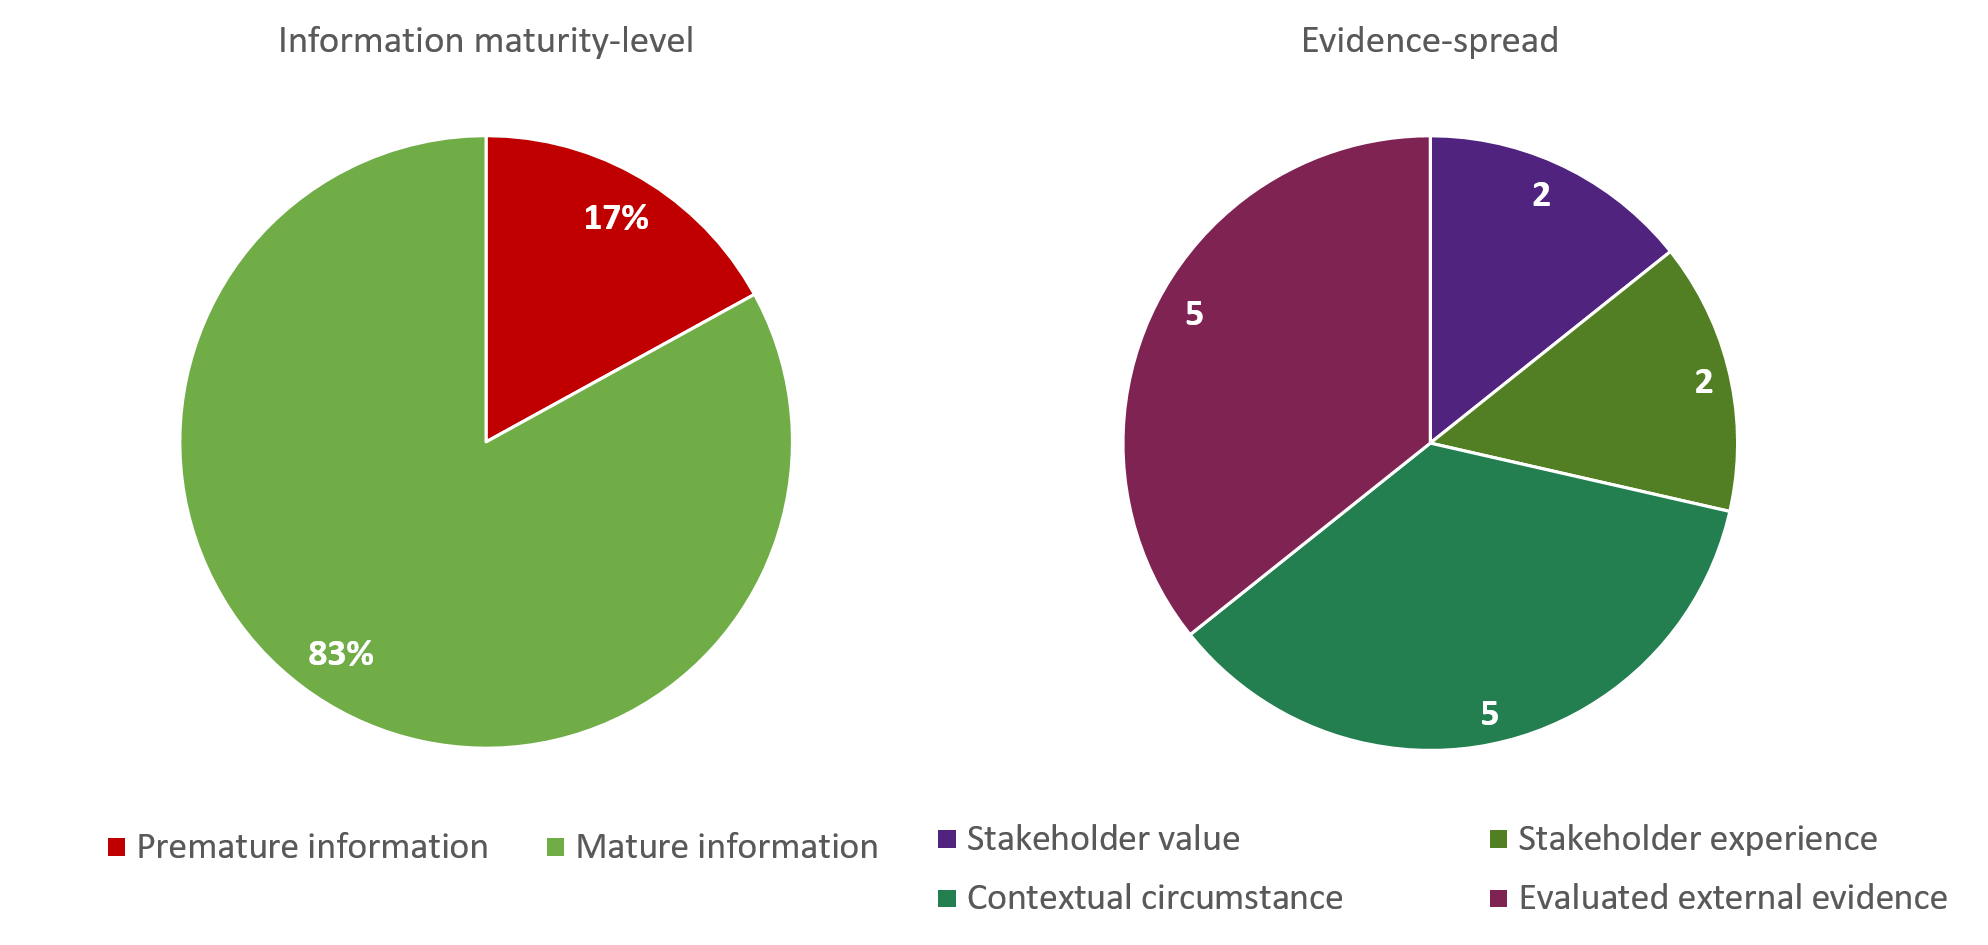
\includegraphics[width=14cm]{../../Images/04_Contribution/Dashboard_Component_1.png}
  \caption{A mock-up of the presentation of the evidence-mix of a specific decision.}
  \label{fig:Dashboard_Component_1}
\end{figure} 

The decision-maker can navigate to the second dashboard by clicking on the pie chart that presents the information maturity-level. Alternatively, the decision-maker can navigate to the third dashboard by clicking on the pie chart that presents the evidence-spread.

\subsubsection{Dashboard 2: Information maturity-level in detail}
The goal of the second dashboard is to enable a decision-maker to understand the consolidated information maturity-level. If the consolidated information maturity-level is lower than expected, the decision-maker can use the second dashboard to understand the root cause. This understanding allows the decision-maker to define actions to improve the information maturity-level. For example, the decision-maker needs to spend time on expanding the information if the completeness pattern causes a low information maturity-level. However, the decision-maker should understand the conflicts and reconsider using conflicting evidence sources if these evidence sources cause a low information maturity-level.

\paragraph{Pattern information maturity-levels}
The detailed information maturity-level consist out of the maturity-level for the completeness, reproducibility, consensus, and conflict patterns. We have defined the functions $mv_1$, $mv_2$, $mv_3$, and $mv_4$ for this. 

In addition to the actual violations $av$, we define $av_1(RI) \Rightarrow \mathbb{N}$, $av_2(RI) \Rightarrow \mathbb{N}$, $av_3(RI) \Rightarrow \mathbb{N}$, and $av_4(RI) \Rightarrow \mathbb{N}$ to represent the actual violations for the completeness, reproducibility, consensus, and conflict patterns. We also define the $avi_x(ri)$ functions that represent the actual violations that a decision-relevant individual generates. Equation \ref{eq:information_maturity_level_x} presents the information maturity-level of the decision-relevant root individuals $RI$ for one of the patterns.

\begin{equation} \label{eq:information_maturity_level_x}
iml_x(RI) = \dfrac{mv_x(RI)-av_x(RI)}{mv_x(RI)}
\end{equation}

\paragraph{Detailed information maturity-level dashboard}
Equation \ref{eq:information_maturity_level_x} defines four pattern-specific information maturity-levels. The pie-chart is most suitable to present percentages and relative proportions \parencite{OTH09}. Figure \ref{fig:Dashboard_Component_2} presents an example of a dashboard that contains the pie charts that present the pattern-specific information maturity-levels. We have made the pie charts easy to understand by tailoring the scales to the specific pattern, representing \emph{good} (the mature information) and \emph{bad} (the premature information) as \textcolor{LightGreen}{green} and \textcolor{Red}{red}, and using data labels. The decision-maker can navigate to the third dashboard by clicking on one of the pie charts. 

\begin{figure}[H]
\centering
  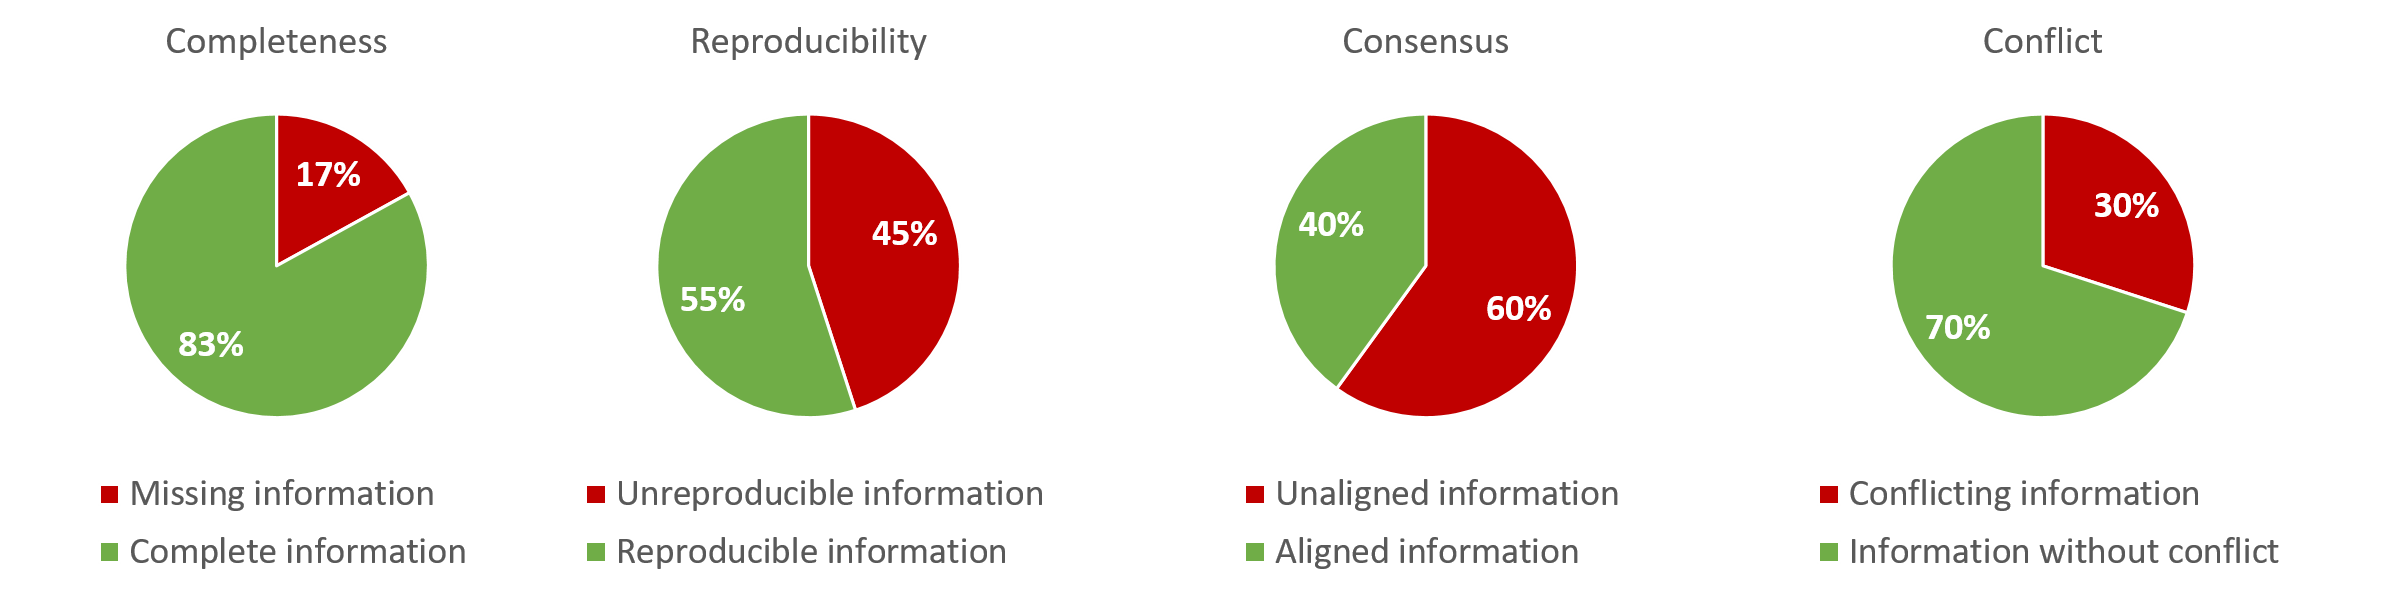
\includegraphics[width=17cm]{../../Images/04_Contribution/Dashboard_Component_2.png}
  \caption{A mock-up of the presentation of the pattern-specific information maturity-levels.}
  \label{fig:Dashboard_Component_2}
\end{figure} 

\subsubsection{Dashboard 3: Violations}
The goal of the third dashboard is to enable the decision-maker to understand which individuals cause the lowered information maturity-level and the evidence spread. The decision-maker might have the following questions:
\begin{enumerate}
\item How can I diversify the evidence types to increase the information maturity-level?
\item Which information is missing?
\item Which information is unreproducible or does not meet the consensus-level?
\item Which information has evidence conflicts?
\end{enumerate}

The answer to these questions allows the decision-maker to increase the information maturity-level. The decision-maker can complete information by entering new information, can reproduce information by linking it to existing or new evidence sources, or remove conflict by discarding information or replacing evidence sources. We focus on the data structure, detection mechanisms, and data presentation. Creating forms to enter new information or change existing information is, therefore, not in the scope of this study. 

We tailor the presentation of the third dashboard, depending on these four questions. The structure of the presented information is similar for the four use-cases. The level of detail requires us to present the information per individual. As a result, we need to present multiple individuals in the same environment. We only present premature individuals to prevent overwhelming the decision-maker with information. Presenting the mature individuals does not make it easier for the decision-maker to answer the questions mentioned earlier.

We want the decision-maker to see the difference between the categories of information in each of the four questions, for example, complete versus incomplete. Presenting the diversity of evidence types for multiple individuals requires four categories: evaluated external evidence, stakeholder value, stakeholder experience, and contextual circumstances. A bar chart allows the decision-maker to compare data across categories \parencite{OTH09}. 

\paragraph{Individual dashboard}
Figure \ref{fig:Dashboard_Component_3_Completeness} presents an example of the presentation of the completeness maturity-level of four individuals. We show the completeness maturity-level for each individual using a bar chart. The number of individuals depends on the scope of the decision. We present the related violations in a table below the bar chart for the selected decision. Even though entering or changing information is not in the scope of this study, we can easily imagine that clicking on one of the violations would direct the decision-maker to a form that allows the decision-maker to enter or adjust information and, as a result, solve the violation immediately. We use the same presentation for the reproducibility, consensus, and conflict-related questions. However, we replace the header of the chart and the name of the data series.

\begin{figure}[H]
\centering
  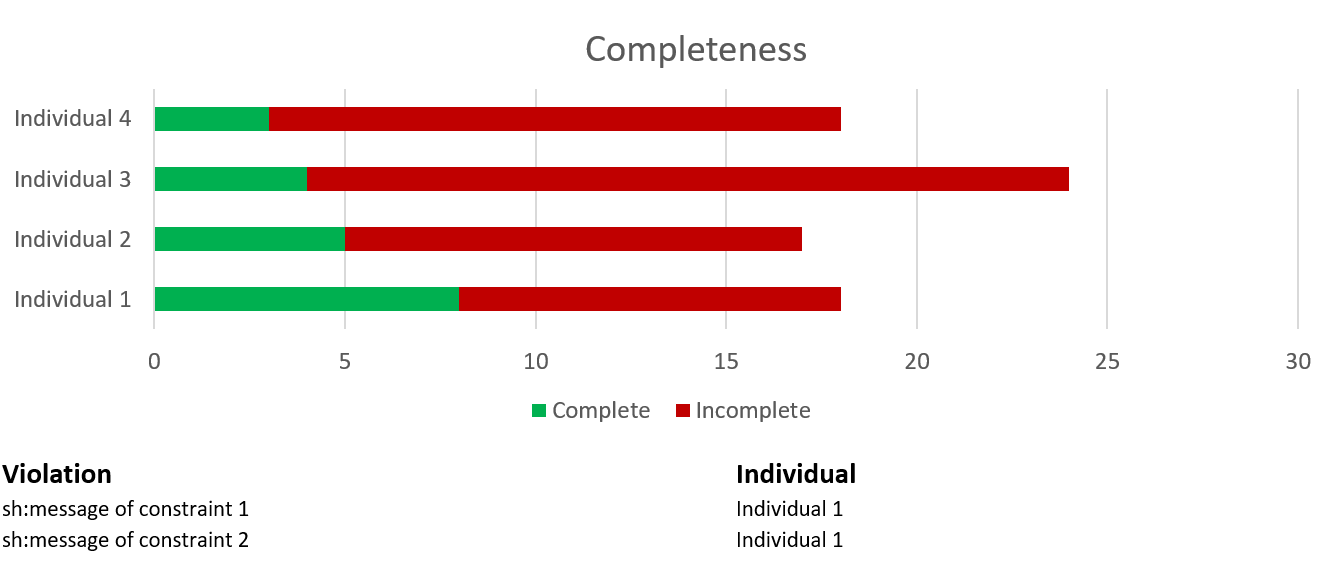
\includegraphics[width=16cm]{../../Images/04_Contribution/04_DecisionPresentationPattern_Component3_Example_Completeness.png}
  \caption{A mock-up of the presentation of the completeness maturity-level of four individuals. We show the completeness maturity-level for each individual using a bar chart.}
  \label{fig:Dashboard_Component_3_Completeness}
\end{figure} 

We extract the actual individual violations from the ontology. The $mvi_1$, $mvi_2$, $mvi_3$, and $mvi_4$ functions define the maximum number of violations per individual. We subtract the actual violations $av$ from the maximum violations $mv$ to get the information without conflict, the complete information, the reproducible information, and the aligned information.

\paragraph{Evidence spread dashboard}
The presentation of the evidence spread is a bit different. Instead of two data series, we need four data series: one for each evidence type. Figure \ref{fig:Dashboard_Component_3_Spread} presents an example of the presentation of the evidence spread of four individuals. We have chosen for a consistent colouring scheme, considering figure \ref{fig:Dashboard_Component_1}. We present the evidence spread for each individual using a bar chart. There are no constraints that enforce a specific evidence spread. Therefore, there are no violations to present. Instead, we present a list of evidence related to the selected individual below the bar chart. Furthermore, we consolidate the list of violations based on the root individuals. This presentation allows a decision-maker to understand the evidence spread and actual evidence related to a root individual. 

\begin{figure}[H]
\centering
  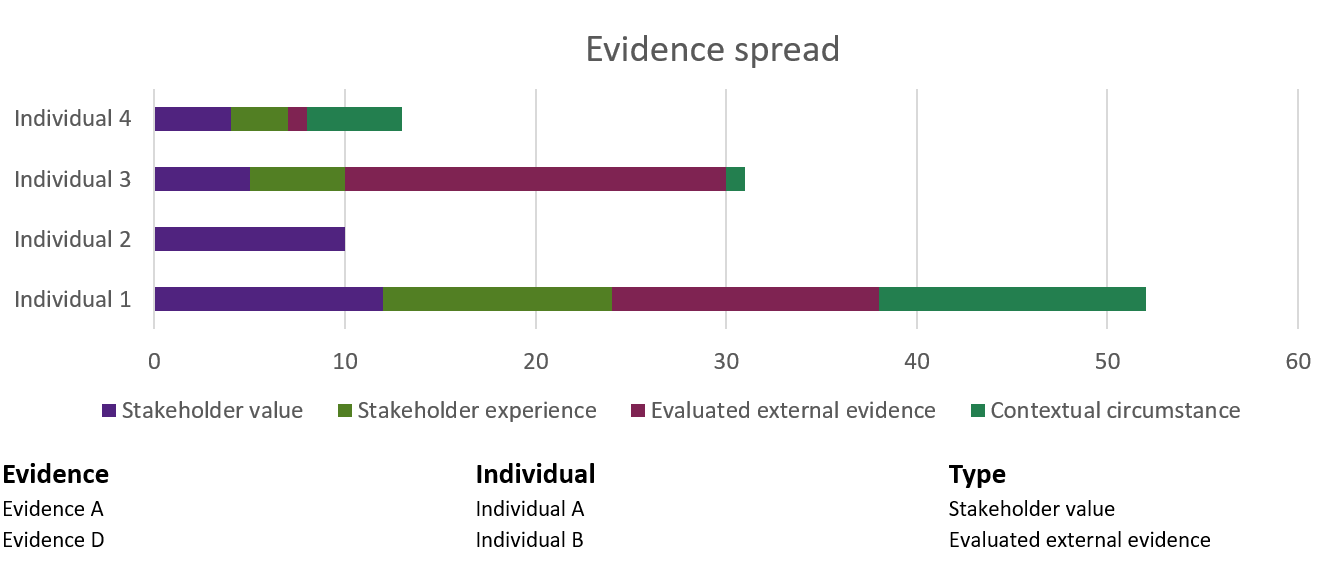
\includegraphics[width=16cm]{../../Images/04_Contribution/04_DecisionPresentationPattern_Component3_Example_Spread.png}
  \caption{A mock-up example of the presentation of the evidence spread of four individuals. We have chosen for a consistent colouring scheme, considering figure \ref{fig:Dashboard_Component_1}. We present the evidence spread for each individual using a bar chart.}
  \label{fig:Dashboard_Component_3_Spread}
\end{figure} 

We considered using an alternative presentation based on graphs. Figure \ref{fig:Dashboard_Component_3_Alternative} presents an example of this presentation. The graph-based presentation overwhelms the decision-maker with a lot of details, including the relationships between decision-relevant information and their status. This example presents only seven decision-relevant individuals. A more extensive example increases the size and complexity of the presentation. Additionally, the edges do not add useful information for the decision-maker.

\begin{figure}[H]
\centering
  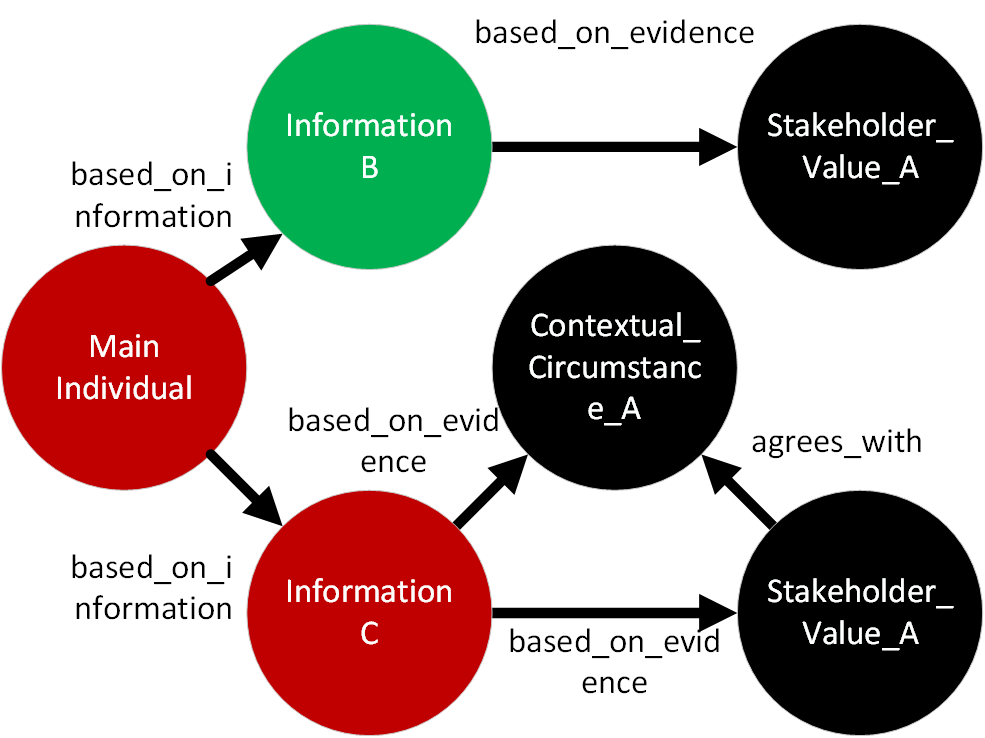
\includegraphics[width=7cm]{../../Images/04_Contribution/04_DecisionPresentationPattern_Component3_Example_Alternative.png}
  \caption{An alternative, more complex, presentation of the decision-relevant individuals and their maturity status.}
  \label{fig:Dashboard_Component_3_Alternative}
\end{figure} 